\section{Convergence Analysis}

Given that the result of \hogwild, in the absence of noise generated by the
asynchronous updates of $x$, henceforth denoted {\it asynchronous noise}, is
equivalent to a stochastic gradient method, we should expect convergence rates
similar to those of stochastic gradient, should noise be small. Take for example
the typical linear least squares loss function $f(x) = \frac{1}{2n}
\norm{Dx-b}_2^2$, where $x \in \mathbb{R}^n$ and $D \in \mathbb{R}^{n \times n}$
a diagonal matrix. Writing this as a sum of each data entry:
\[
  f(x) 
  = \frac{1}{2n} \sum_{k=1}^n (D_{ii}x_i - b_i)^2
  = \frac{1}{n} \sum_{k=1}^n f_i(x)
  \implies
  (\nabla f_i(x))_k
  =
  \begin{cases}
    D_{ii}(D_{ii}x_i - b_i), & k = i \\
    0, & k = 0
  \end{cases}
\]
Because our $\nabla f_i(x)$'s only have a single entry in their own component, we
can see that as long as no other thread is working on component $i$
simultaneously, no asynchronous noise will be generated; should we use \hogwild\
without replacement then this is guaranteed. In the original paper
\cite{2011NRRW}, sparsity of the vector $\nabla f_i(x)$ was required in order to
guarantee convergence, but as we'll see later, this isn't always necessary.

As a baseline of comparison, we first state a result on the convergence of the
stochastic gradient method:
\begin{theorem} \label{thm:sgd}
  (Convergence of the Stochastic Gradient Method \cite{2016BCN}) Let $F:
  \mathbb{R}^d \to \mathbb{R}$ be an objective function we're seeking to
  minimize. We can write this as either an expected risk $F(x)
  = \mathbb{E}_\xi{f(x, \xi)}$, or an empirical risk $F(x) = \frac{1}{n}
  \sum_{k=1}^n f_k(x)$.  Under the assumptions:
  \begin{enumerate}[(1)]
    \item $F$ is continuously differentiable and $\nabla F$ is Lipschitz
      continuous with Lipshitz constant $L$, i.e.
      \[
        \norm{\nabla F(x) - \nabla F(y)} 
        \leq
        L\norm{x-y}, \forall x,y \in \mathbb{R}^d
      \]
    \item $F$ is strongly convex with constant $c$, i.e.
      \[
        F(x) \geq F(y) + \nabla F(y)^T (x-y) + \frac{1}{2}c\norm{x-y}^2, 
        \forall x,y \in \mathbb{R}^d
      \]
    \item $F$ is bounded below over the region explored by stochastic gradient
      method.
    \item In expectation, the vector $-\nabla f(x_k, \xi_k)$ is a descent
      direction for $F$ with norm bounded by it's own norm. That is: $\exists
      \mu_G \geq \mu > 0$ such that $\forall k \in \mathbb{N}$:
      \[
        \nabla F(x_k)^T \E{\nabla f(x_k,\xi_k)} \geq \mu \norm{\nabla F(x_k)}^2
        \text{ and }
        \norm{ \E{\nabla f(x_k,\xi_k)} } \geq \mu_G \norm{\nabla F(x_k)}
      \]
    \item $\exists M, M_V \geq 0$ such that $\forall k\in \mathbb{N}$:
      \[
        \Var{\nabla f(x_k, \xi_k)} \leq M + M_V \norm{\nabla F(x_k)}^2
      \]
  \end{enumerate}
  Then, assuming a fixed stepsize $\alpha$ (a.k.a. learning rate), satisfying
  $\alpha \in (0, \mu/ LM_g]$, we have:
  \[
    \E{F(x_k) - F_*} 
    \leq 
    \frac{\alpha LM}{2c\mu} + (1 - \alpha c \mu)^{k-1}
    \left(
      F(x_1) - F_* - \frac{\alpha LM}{2c\mu}
    \right)
  \]
  and if we instead choose $\alpha$ diminishing, i.e. let $\alpha_k
  = \frac{\beta}{\gamma + k}$ where $\beta > 1/c\mu, \gamma > 0$ are chose such
  that $\alpha_1 \leq \mu/LM_G$, then:
  \[
    \E{F(x_k) - F_*} 
    \leq 
    \frac{1}{\gamma + k} \max
    \left\{
      \frac{\beta^2 LM}{2(\beta c \mu -1)},
      (\gamma + 1)(F(x) - F_*)
    \right\}
  \]
\end{theorem}
The result is technical, and very long to prove, so I just refer to the article
\cite{2016BCN} for it. Regardless, the last result in the above theorem is what
we strive for in $\hogwild$: convergence in $\mathcal{O}(1/k)$ time.

\subsection{Theoretical Results}

\hogwild's original article \cite{2011NRRW} manages to prove that the
asynchronous noise generated by \hogwild, under certain sparsity assumptions of
the $f_i$'s, converged at the same rate as seen in the stochastic gradient
method. However, a newer article from 2015 by De Sa et al. \cite{2015SZOR}
presented a new framework in the context of martingale theory, which drops said
sparsity assumptions and generalizes to certain non-convex formualations. Given
that I just learned about martingale theory essentially two weeks ago in Basic
Probability, and that much of my synthetic tests are on dense datasets, I feel
compelled to present this argument instead. 

The following is a cleaned up summary of the arguments presented in the article,
except I focus on just demonstrating how martingale theory can be used to
generalize convergence arguments for a sequential stochastic gradient method to
the asynchronous case, and cut out the generalization required for the
non-convex situation.

\subsubsection{Initial Machinery}

First, recall the definition of a martingale:
\begin{definition} \label{def:martingale}
  \cite{2004JP} A sequence of random variables $(X_n)_{n \geq 0}$ is called
  a martingale, or an $(\mathcal{F}_n)$-martingale, if
  \begin{enumerate}[(i)]
    \item $\E{|X_n|} < \infty, \forall n$.
    \item $X_n$ is $\mathcal{F}_n$ measurable, $\forall n$.
    \item $\E{X_n \mid \mathcal{F}_m} = X_m$ a.s., $\forall m \leq n$.
  \end{enumerate}
  furthermore a supermartingale (submartingale) is one satisfying (i), (ii)
  exactly, and (iii) with $\leq\ (\geq)$ instead.
\end{definition}
Using this, the idea is to model our convergence with a non-negative
supermartingale $W_t(x_t, \dots, x_0)$ which is a function of the previous
stochastic gradient iterates. These $W_t$, when used in the theory later, will
be associated with specific stochastic algorithms, as an example below we'll see
it applied to serial stochastic gradient. However, given such a supermartingale,
and given a bounded stopping time $B$ (in literature known as a horizon), if our
stochastic gradient iterates are written as $x_{t+1} = x_t - \eta \nabla
f_t(x_t)$, where $\eta$ is the learning rate, and $f_t$ denotes the random
function chosen at time step $t$, then we see that condition (iii) in the above
definition implies that:
\[
  W_{t+1}(x_t - \eta \nabla f_t(x_t), x_t, \dots, x_0)
  \leq
  W_t(x_t, \dots, x_0), \forall t \leq B
\]
which certainly makes sense if our $-\nabla f_t(x_t)$ is a sufficient search
direction. Furthermore, letting our success region be denoted as $S
= B_\e(x^*)$, where $x^*$ is the minimizer of our optimization problem, if we
impose that if $x_t \not\in S, \forall t \leq T$ then:
\[
  W_T(x_T, \dots, x_0) \geq T
\]
then we call $W_t$ a {\it rate supermartingale}. To simplify notation, let $F_t$
be the event where $\nexists t \leq T$ such that $x_t \in S$. 

A good example of the power of this machinery is proving a convergence bound on
the serial version of stochastic gradient: using (iii) of definition
\ref{def:martingale}, one can see that considering $F_T$:
\[
  \E{W_0(x_0)}
  \underbrace{\geq}
  \E{W_T}
  =
  \Prob{F_t}
  \underbrace{\Prob{F_T}\E{W_T | F_T}}_{W_T \geq T} + 
  \underbrace{\Prob{F_T^c}\E{W_T | F_T^c}}_{W_T \geq 0}
  \geq
  \Prob{F_T}T
\]
where the first inequality is by Doob's optional sampling theorem. Thus for
a simple serial stochastic gradient method: $\Prob{F_t} = \E{W_0} / T$.

Now that we can characterize serial stochastic gradient in this model, we need
a method to analyze asynchronous noise. Recall that since we've guaranteed in
the description of \hogwild\ that writes to the iteration variable $x_t$ are
done atomically, the only race condition possible is when updates to entries of
$x_t$ are interleaved with either the other thread's updates or its reads on
$x_t$.

Indeed, when going to update the $i$th component of $x_{t+1}$, the variable used
to compute the gradient may have long since changed, making our iteration look
more like $x_{t+1} = x_t - \nabla f_t(v_t)$ where $v_t$'s entries were the
entries of some previous iterate $x$. Let $\tau_{i,t}$ denote the lag for the
update of the $i$th component of $x_{t+1}$, i.e. $(v_t)_i = ( x_{t-\tau_{i,t}}
)_i$. Then we recognize that this lag for each component $i$ (supposing the
computer hasn't crashed) must be bounded; let $\tau'$ be the the maximum of such
bounds and let $\tau = \E{\tau'}$. This is known in literature as the {\it
worst-case expected delay}.

Finally, we need one last definition, mainly one of convinience, to proceed
onward. This describes the main conditions upon a rate supermartingale necessary
to prove that the asynchronous noise error is irrelevant to the convergence
rate.
\begin{definition}
  An algorithm with associated rate supermartingale $W$ is $(H, R, \xi)$-bounded
  if the following conditions hold.
  \begin{enumerate}[(1)]
    \item $W$ must be Lipschitz continuous in the current iterate with parameter
      $H$, i.e.
      \[
        \norm{W_t(u, x_{t-1}, \dots, x_0) - W_t(v, x_{t-1}, \dots, x_0)}
        \leq
        H\norm{u-v}, \forall t, u, v, x_t, \dots, x_0.
      \]
    \item $\nabla f$ must be Lipschitz continuous in expectation with parameter
      $R$, i.e.
      \[
        \E{||\nabla f(x) - \nabla f(y)||} \leq R\norm{u-v}
      \]
    \item The expected magnitude of the update must be bounded by $\xi$, i.e.
      \[
        \E{||\nabla f(x)||} \leq \xi
      \]
  \end{enumerate}
  Note that these look very familiar to the conditions in the stochastic
  gradient method convergence theorem (theorem \ref{thm:sgd}).
\end{definition}

\subsubsection{Convergence of \hogwild}

Now that we have

\subsection{Numerical Experiments}
Now that we've finally slogged through the presentation of the theory, we can
produce a few numerical experiments. Take, for example, the linear least squares
regression problem with $A \in \mathbb{R}^{n \times m}, x \in \mathbb{R}^m$ and
$b \in \mathbb{R}^n$:
\[
  f(x) = \frac{1}{2}\norm{Ax-b}_2^2 
  = \sum_{k=1}^n 
  \underbrace{ \frac{1}{2} (A_ix - b_i)^2 }_{f_i(x)}
\]
This is a particularily interesting example, as when we examing the stochastic
descent direction of this loss function:
\[
  \nabla f_i(x) = A_{i*}^T(A_{i*}x - b_i), 
  \text{ where }
  A = 
  \begin{bmatrix}
    A_{1*} \\
    \vdots \\
    A_{n*}
  \end{bmatrix}
\]
we notice that the sparsity pattern of $\nabla f_i(x)$ is entirely controlled by
by the sparsity pattern of the rows of $A$. This makes this problem
particularily convinient when trying to understand the effect of sparsity on the
asynchronous noise generated by \hogwild. The original paper \cite{2011NRRW}'s
results required strict assumptions on the sparsity pattern of $\nabla f_i(x)$
in order to guarantee convergence, but as we saw in Theorem
\ref{thm:convexconv}, as long as certain regularity properties are satisfied,
there's no need for such an assumption. Indeed $f$ does satisfy the above,
assuming that $A$ is of full rank%
\footnote{
  One subtle note is that the second condition is actually equivalent to having
  upper bounded maximal eigenvalue. I think we proved this back when we were
  discussing Nesterov's method, and also can be found at this stackexchange
  \url{https://math.stackexchange.com/a/1699082/245618}.
}. Therefore, when $A$ is both sparse and dense, we should see
a $\mathcal{O}(1/k)$ convergence rate, and indeed see figure
\ref{fig:convergence} for the validation of that.
\begin{figure}[!htb]
  \centering
  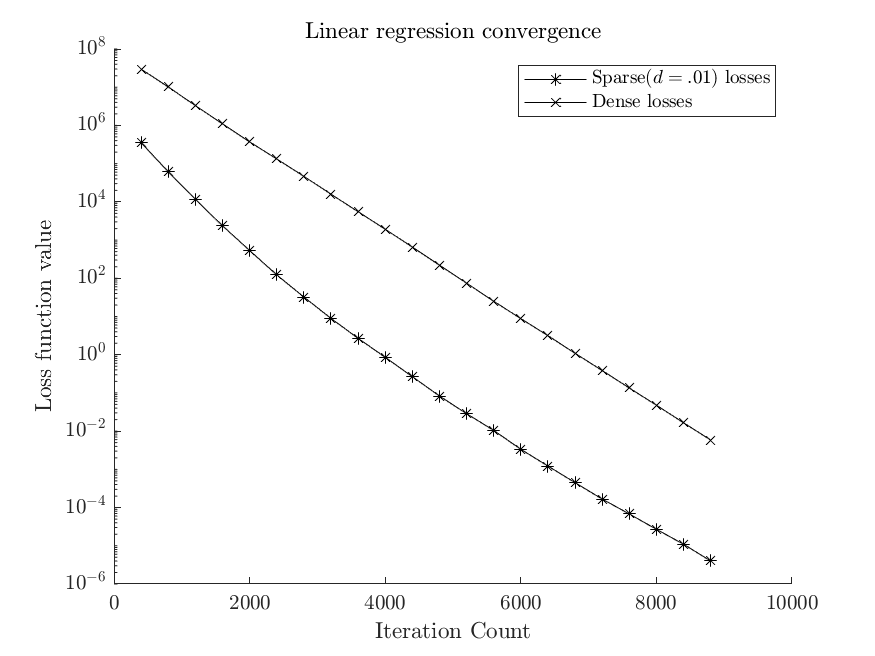
\includegraphics[width=.8\textwidth]{./resources/convergence}
  \caption{
    The matrix Sparse$(d = 0.1)$ is generated by the command {\tt
    sprand(n,m,.01)}. Playing with the density parameter doesn't change the
    shape of the convergence line, but note that denser matrices (since the
    entries are Gaussian) produce a higher initial loss and suffer from more
    asynchronous noise, and therefore require more iterations.
  } \label{fig:convergence}
\end{figure}


